\label{tnp_procedure}\\
\par Simulation studies are important to validate the measurements on data. However, there are possibilities that the studies based on the
simulations can be biased due to some insufficient event description and the lack of understanding of the detector.
Further, for an analysis we always optimize the the event selection and in an ideal selection, we efficiently eliminate the background events with optimal signal events. 
Every real selection affects signal efficiencies which should be estimated.
These efficiencies can be extracted directly from the simulation, but there is a danger such as bias which can appear as mentioned above.
Such bias from MC,  can be estimated by measuring the selection efficiencies directly from the experimental data.
In high purity environment, one can measure the efficiencies by cut and cout method; however, if significant background is involved one needs to measure the efficiencies by  ``fit method'' i.e. by using the Tag-and-Probe (TnP) method. 

The TnP Tool is a generic tool developed to measure any user defined object efficiency (e.g. in this dissertation the reconstruction and/or identification, impact parameter cuts isolation and trigger) from data or MC by expoiting the di-object resonances like $Z$, $\jpsi$ or $\Upsilon$ \cite{pog_tnp}. % https://twiki.cern.ch/twiki/bin/view/CMSPublic/TagAndProbe 
Z boson decaying to a lepton pair is considered to be standard candle for the measurement of these efficiencies (except for reconstruction and identification of  muons at low $\pt$ (i.e. $\pt<20 \GeV$) where $\jpsi$ resonances are used). 
Brief description of the procedure is given as under:

\begin{itemize}
\item Resonances are reconstructed as pairs with one leg passing a tight selection (called ``tag'') and one passing a loose selection (called ``probe'').
\item According to whatever efficiency to be measured, passing probes (from all probes) are defined if they also pass the selection. Those which do not pass the selection are call ``failing probes''.
\item Di-leptons mass distributions are built using ``tag + passing probes'' and ``tag + failing probes'', and are separately fit using ``signal + background'' model.
\item The ratio of the signal yields in these two lineshapes give the subject ``efficiency''.
\item The procedure is repeated in bins of probe variables (i.e. $\pt, \eta$ and so on) to visualize the efficiencies in response of varying these variables.
\end{itemize}
\\
An example of a TnP fit is shown in the Figure. \ref{fig:tnp_fit_example}. And schematic workflow of the TnP method while performing the procedure in measurements using the CMS central framework is shown in the Figure. \ref{fig:tnp_workflow}.

\begin{figure}[!htb]
\vspace*{0.3cm}
\begin{center}
%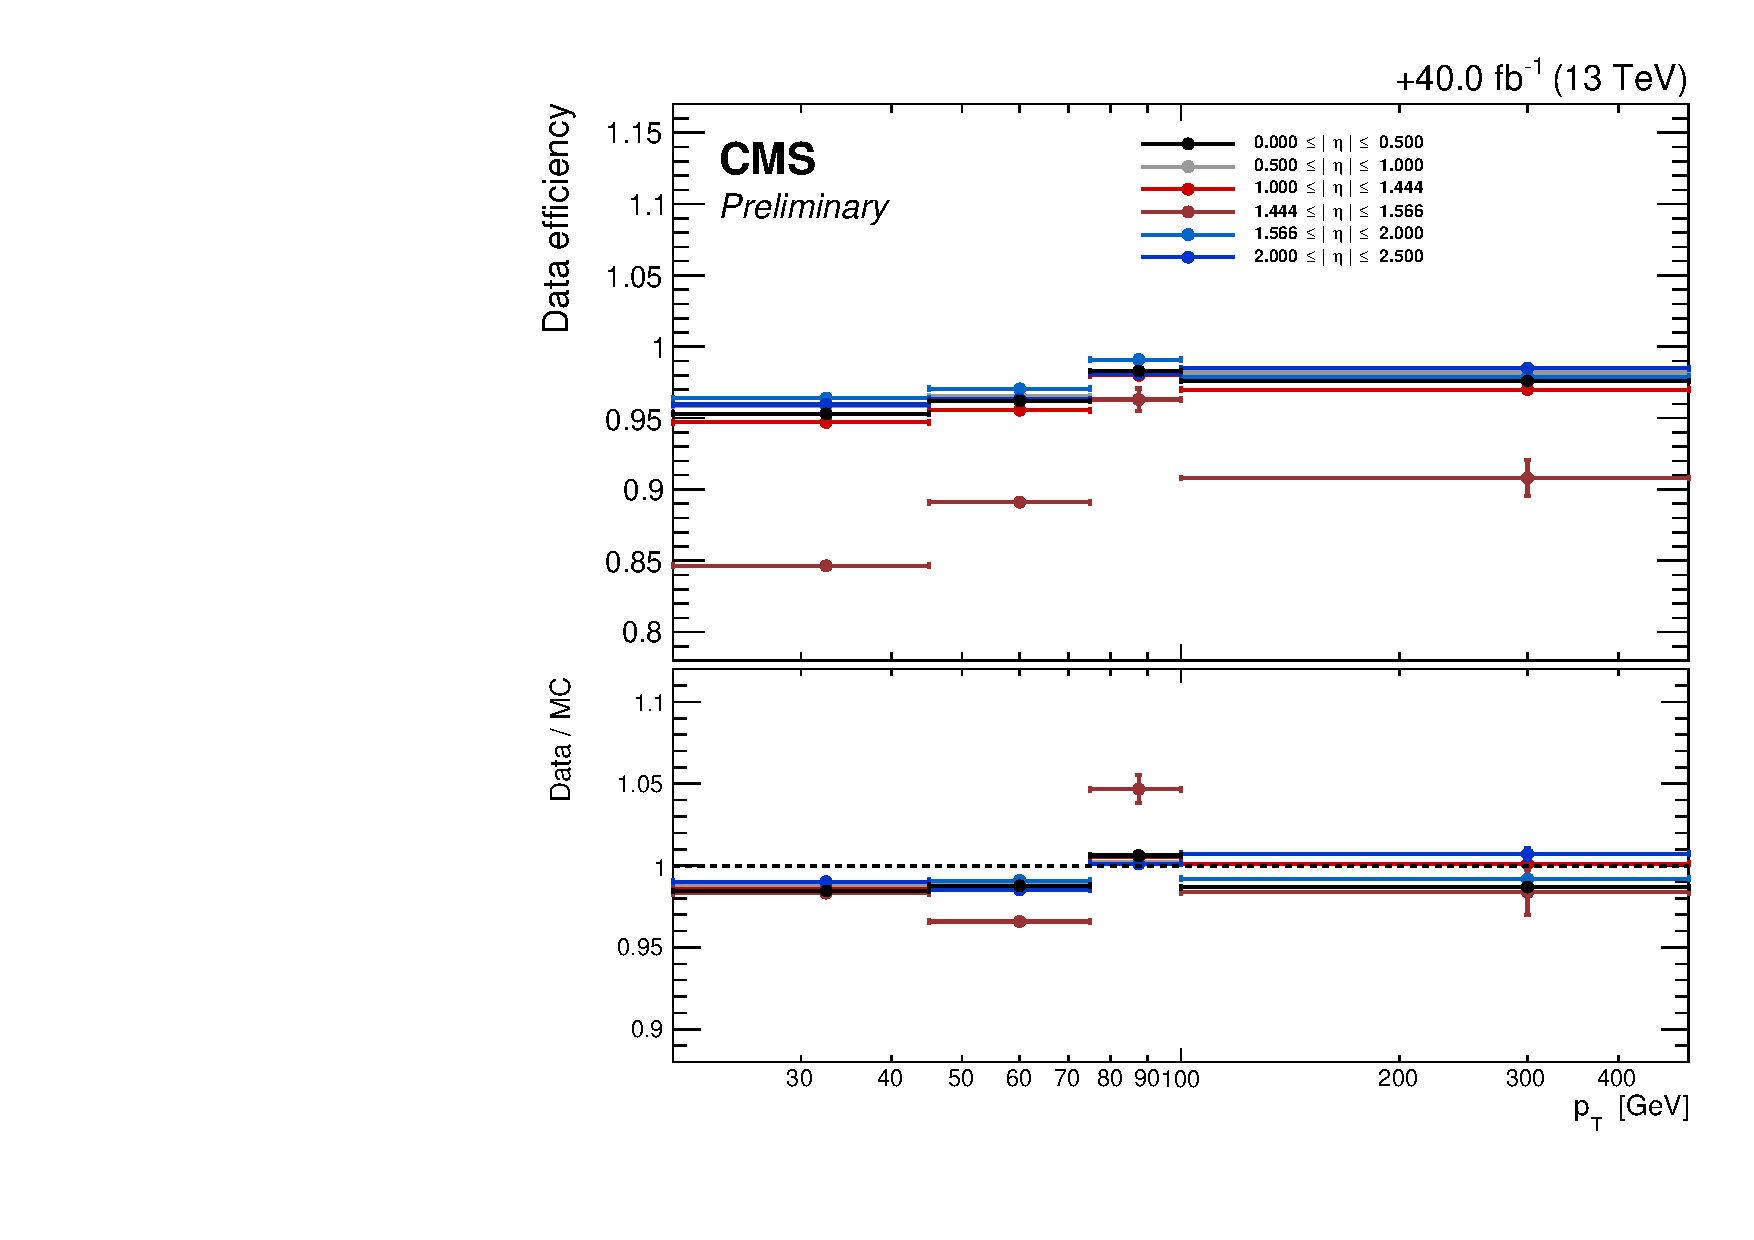
\includegraphics[width=0.4\textwidth]{Figures/Electrons/ErecoPt}
%\includegraphics[page=2, width=0.4\textwidth]{Figures/Electrons/ErecoEta}\\
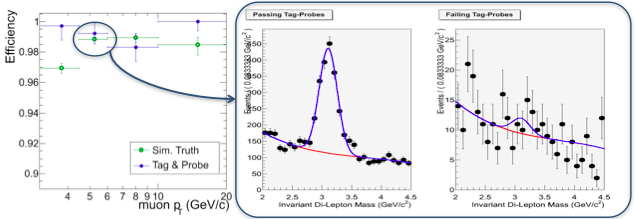
\includegraphics[width=1.0\textwidth]{Figures/tnp_fit_example1.png}
%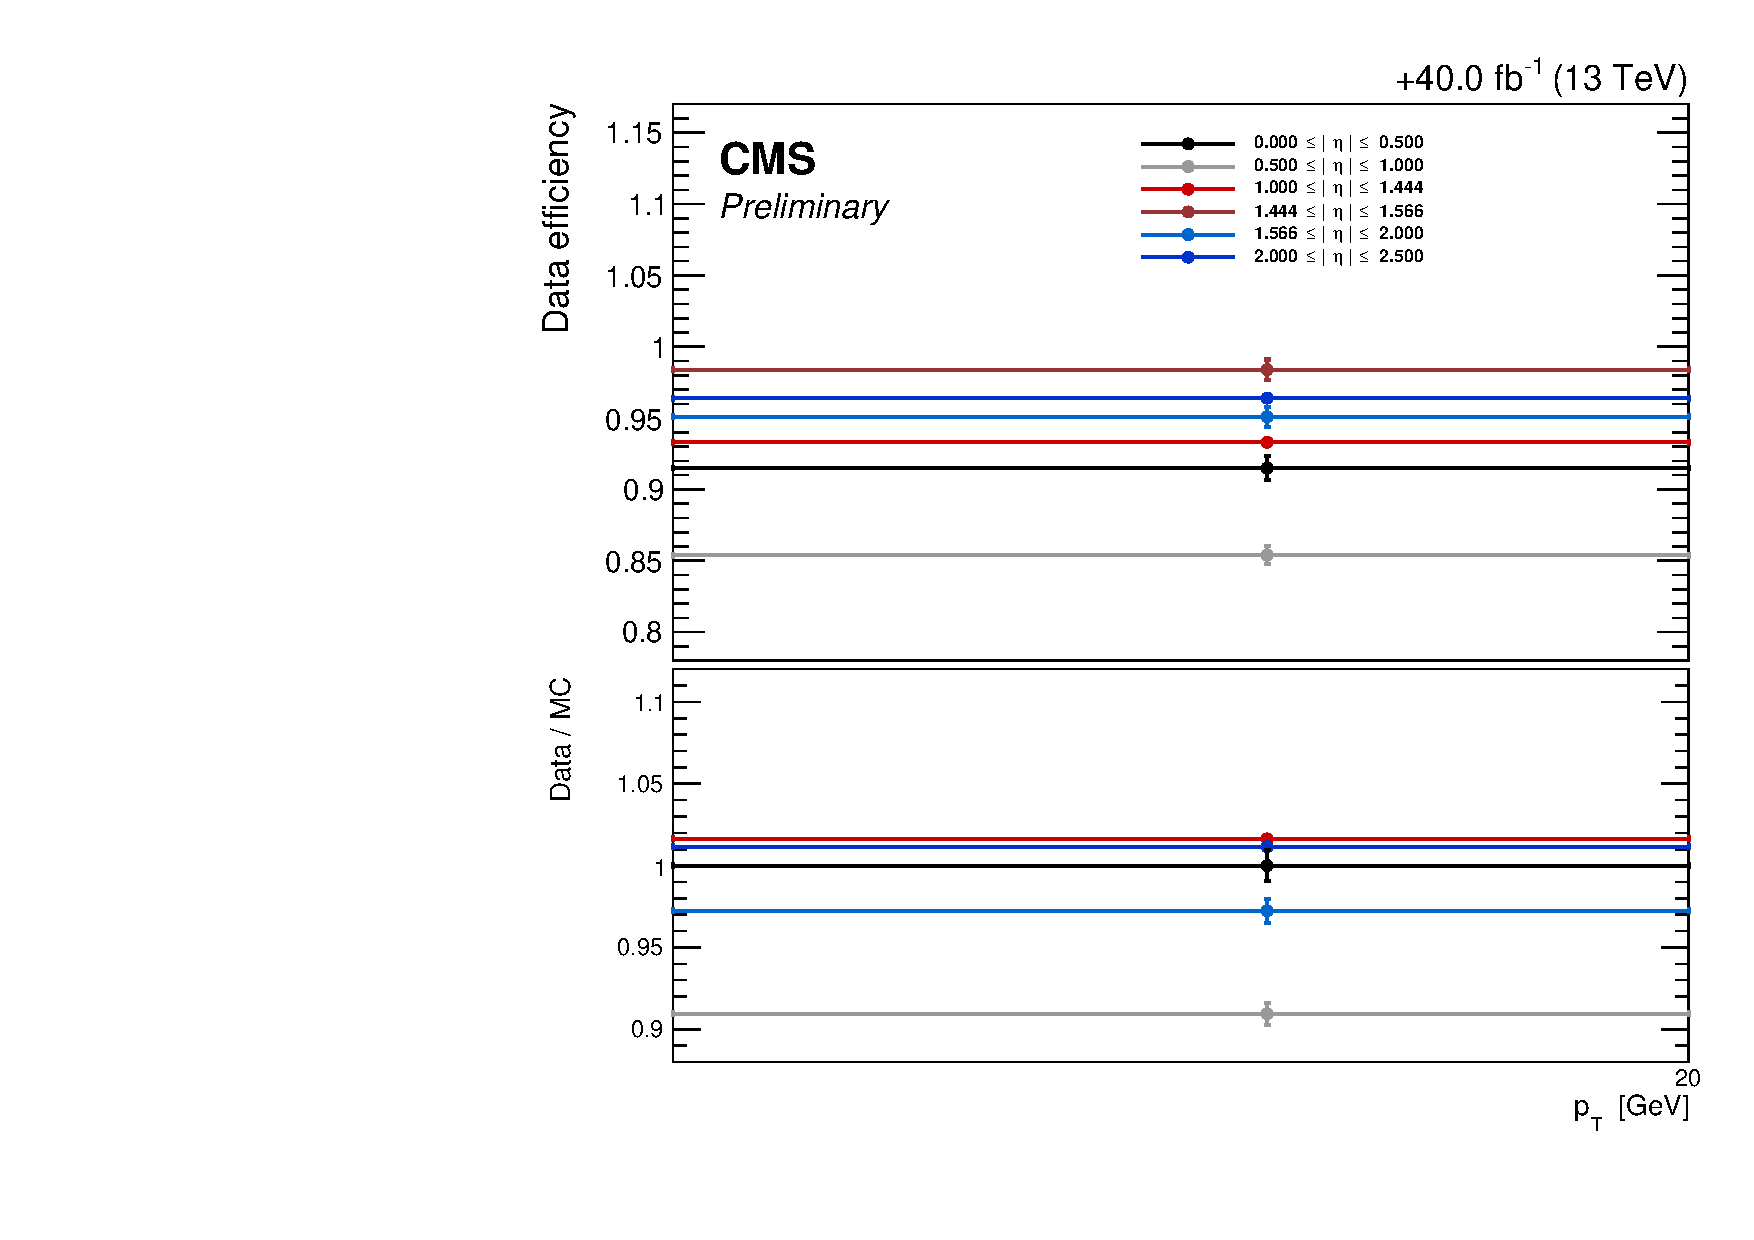
\includegraphics[width=0.4\textwidth]{Figures/Electrons/ErecoEta_lowPt}
\end{center}
	\caption{Efficiency plots in bins of $\pt$ alongwith an example of TnP fit of di-lepton distributions. In the fit plot, black points are data points with statistical uncertainty bars, red lineshape is background fit and blue lineshape is ``signal+background'' fit in case of ``tag + passing probes'' (left) and ``tag + failing probes'' (right)}
\label{fig:tnp_fit_example}
\end{figure}


\begin{figure}[!htb]
\vspace*{0.3cm}
\begin{center}
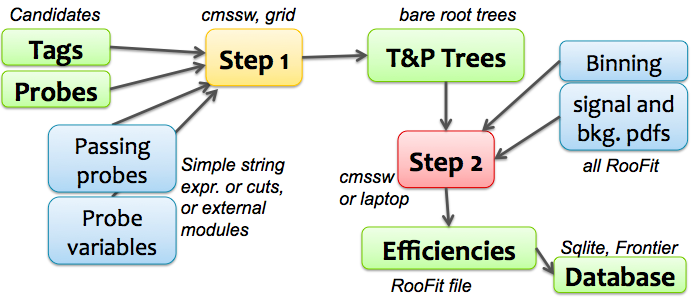
\includegraphics[width=.85\textwidth]{Figures/tnp_workflow.png}
\end{center}
        \caption{Tag and Probe workflow example using the central CMS framework.}
\label{fig:tnp_workflow}
\end{figure}




%%In the case of electron efficiency measurements, this method exploits Z ! e+e− events
%
%308 to estimate the reconstruction and selection efficiencies
%
%The Tag-and-Probe study was performed on the EGM dataset using the golden JSON of ~58.83, 41.4 and 35.9 fb$^{-1}$ respectively for 2018, 2017 and 2016. More details on this technique can be found in Ref.~\cite{AN-15-277}. 
%
%Tag electrons need to satisfy the following quality requirements:
%\begin{itemize}
%%\item trigger matched to HLT\_Ele27\_eta2p1\_WPTight\_Gsf\_v*
%\item trigger matched to HLT\_Ele32\_WPTight\_Gsf\_L1DoubleEG\_v*
%\item $p_{T} > 30$~GeV, super cluster (SC) $\eta < 2.17$% but on in EB-EE gap ($1.4442<|\eta|<1.566$)
%%\item tight working point of the Spring16 cut-based electron ID
%\end{itemize}
%
%For the bin between 7 and 20 GeV, additional criteria are required: the tag has to pass a cut on the MVA ID$>0.92$, $\sqrt(2*PFMET*p_T(tag)*(1-cos(\phi_{MET}-\phi_{tag})))<45 GeV$.
%
%Probe electrons only need to be reconstructed as GsfElectron while the FSR recovery algorithm is not applied in efficiency measurement. 
%
%
%The nominal MC efficiencies are evaluated from the LO MadGraph Drell-Yan, while the NLO systematics use the MadGraph\_AMCatNLO sample.
%
%For the efficiency measurements a template fit is used. The $m_{ee}$ signal shape of the passing and failing probes is taken from MC and convoluted with a Gaussian. The data is then fitted with the convoluted MC template and a CMSShape (an Error-function with a one-sided exponential tail). This change follows from the usage of the T\&P tool developed by the EGM POG.
%
%
%%\paragraph{Electron selection efficiency measurements}\mbox{}\\
%%\label{par:Efficiency_measurements}
%
%The measurement of electron selection efficiency is made as a function of the probe electron $p_{T}$ and its SC $\eta$. For electrons falling in the ECAL gaps, it is measured separately. Figure \ref{fig:ele_sel_pt_turn_on} and \ref{fig:ele_ele_eta_turn_on} shows the $p_{T}$ and $\eta$ turn-on curves measured in data.
%% and the final 2D scale factor is shown in Fig.~\ref{fig:ele_sel_scale_factors} together with the systematic uncertainties. %These scale factors are very similar to the ICHEP figures, but more homogenous across $\eta$ and $p_{T}$ because of the higher statistics and the usage of more stable fitting routines in the new T\&P tool.
%
%
%\begin{figure}[!htb]
%\begin{center}
%    \subfigure [] {\resizebox{7.5cm}{!}{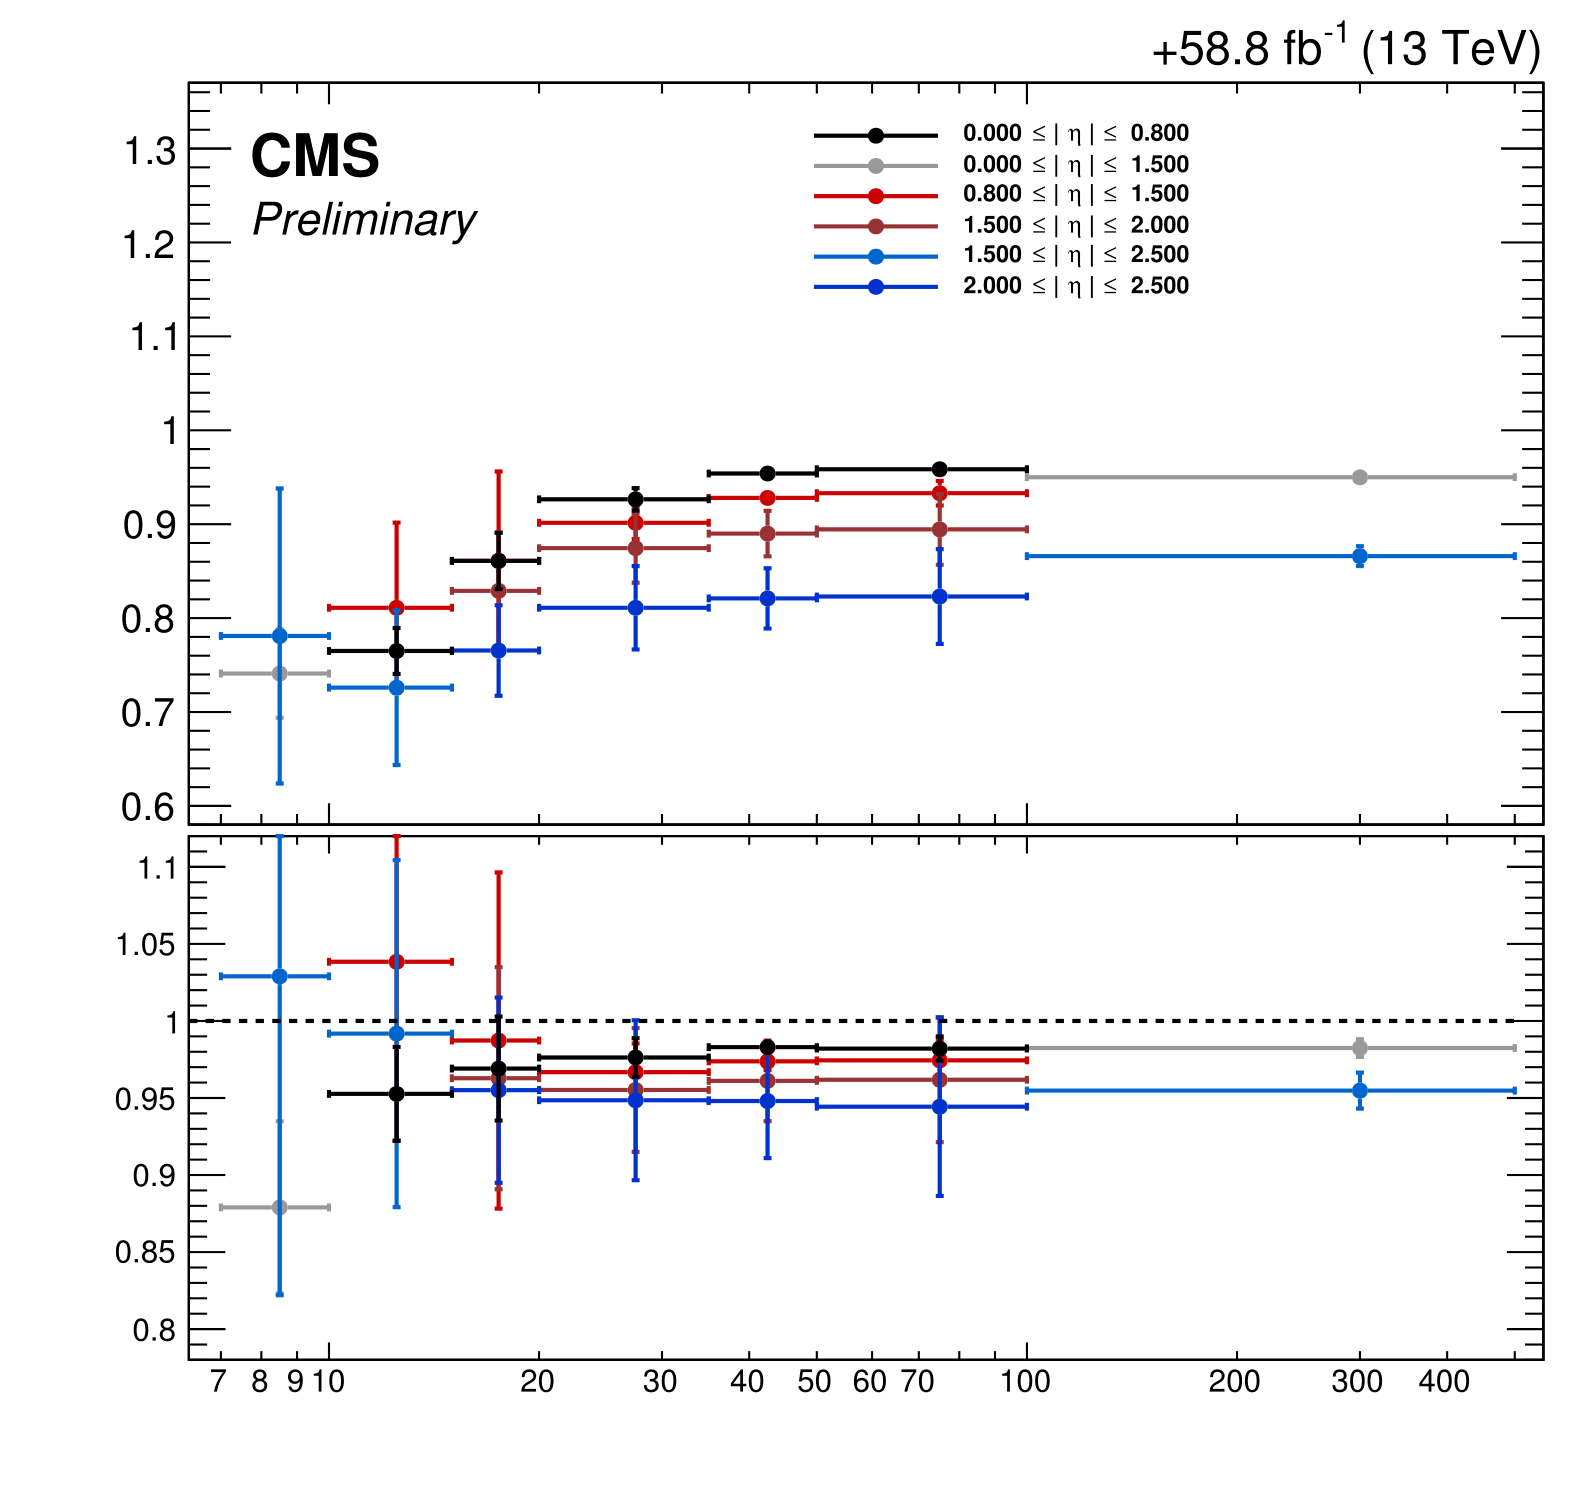
\includegraphics{Figures/Electrons/eleSFvspT.png}}}
%    \subfigure [] {\resizebox{7.5cm}{!}{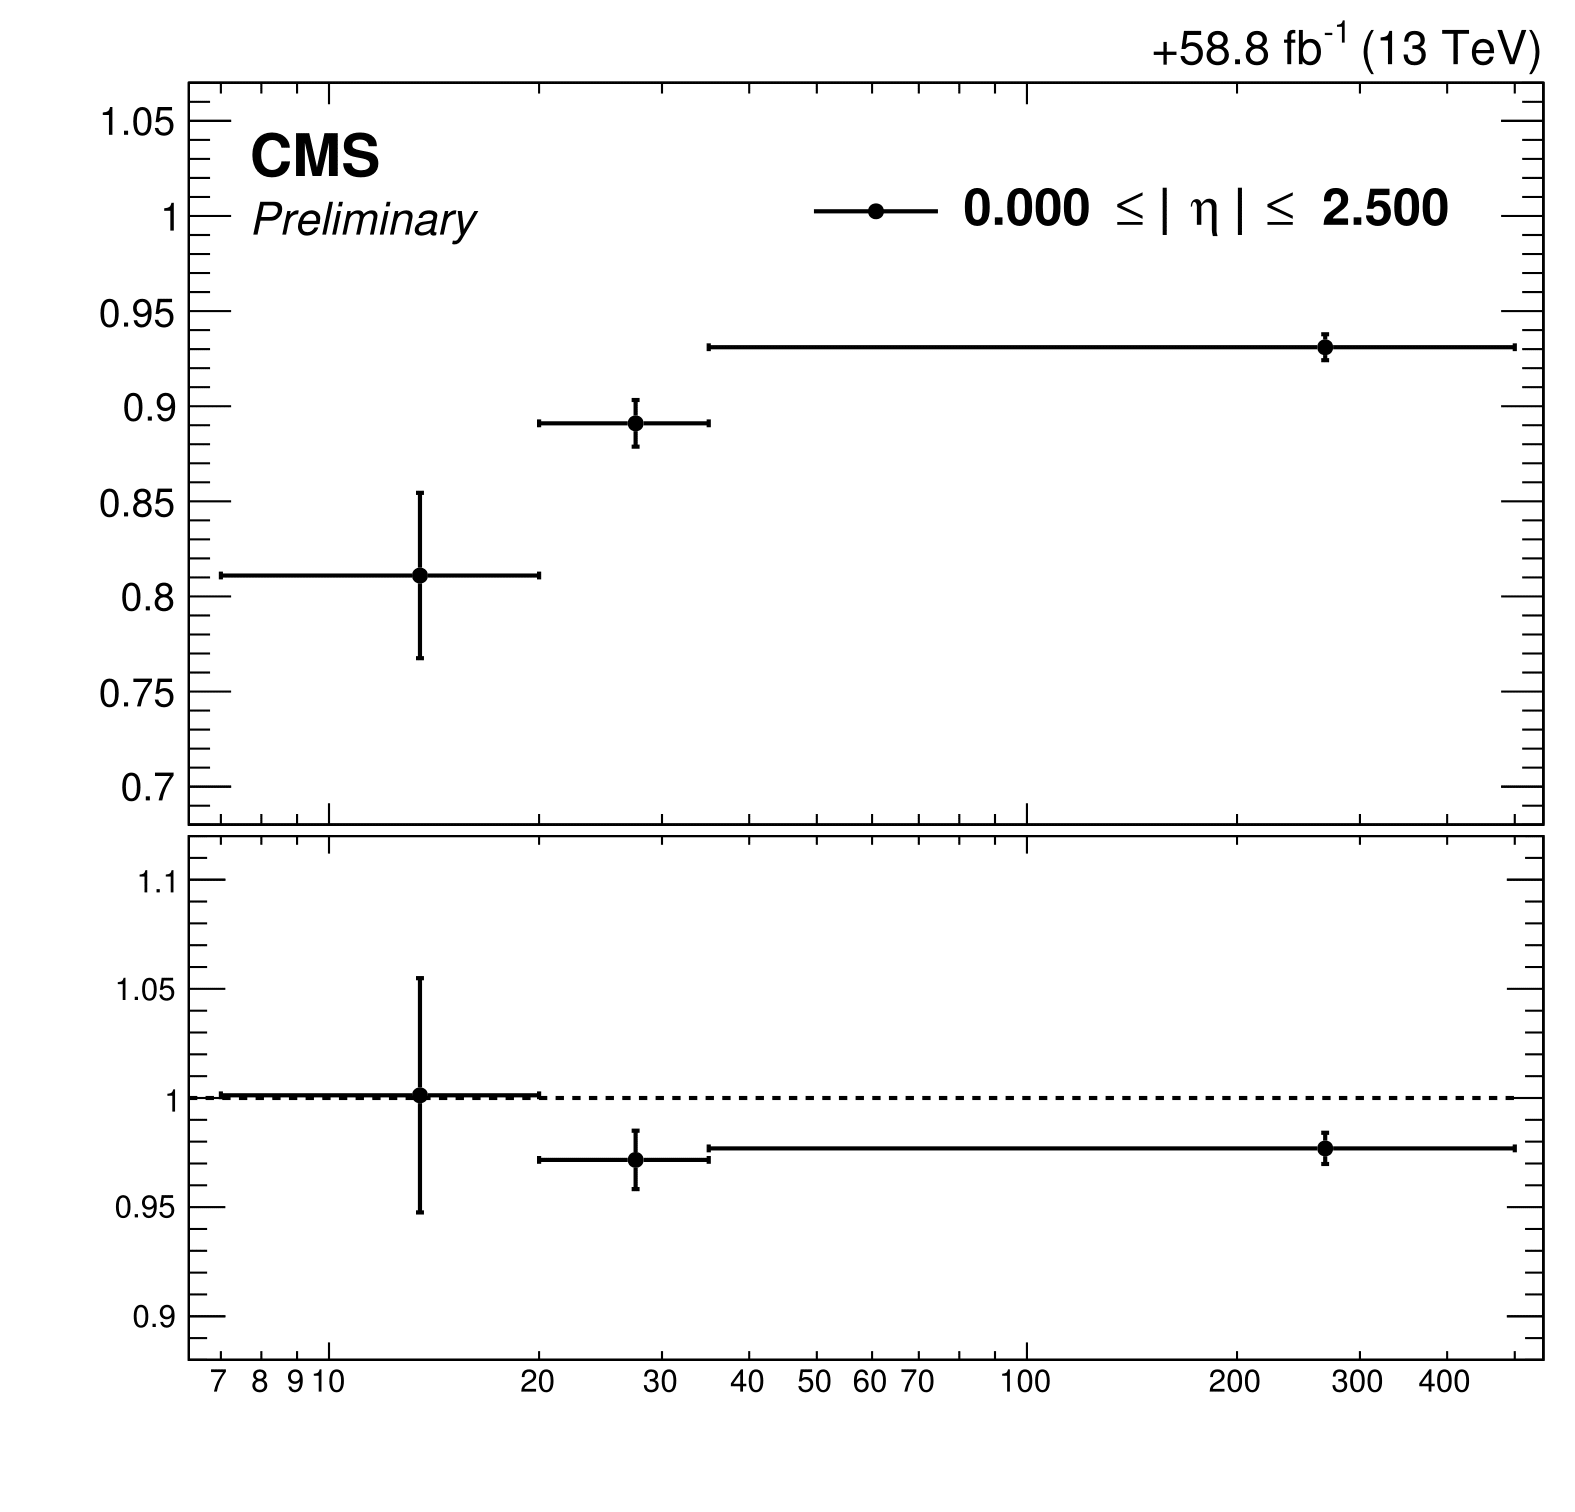
\includegraphics{Figures/Electrons/eleSFvspTgap.png}}}\\
%\caption{Electron selection efficiencies vs $p_T$ measured using the Tag-and-Probe technique, non-gap electrons (left) and gap electrons (right), together with the corresponding data/MC ratio bottom part of each plot.}
%\label{fig:ele_sel_pt_turn_on}
%\end{center}
%\end{figure}
%
%\begin{figure}[!htb]
%\begin{center}
%    \subfigure [] {\resizebox{7.5cm}{!}{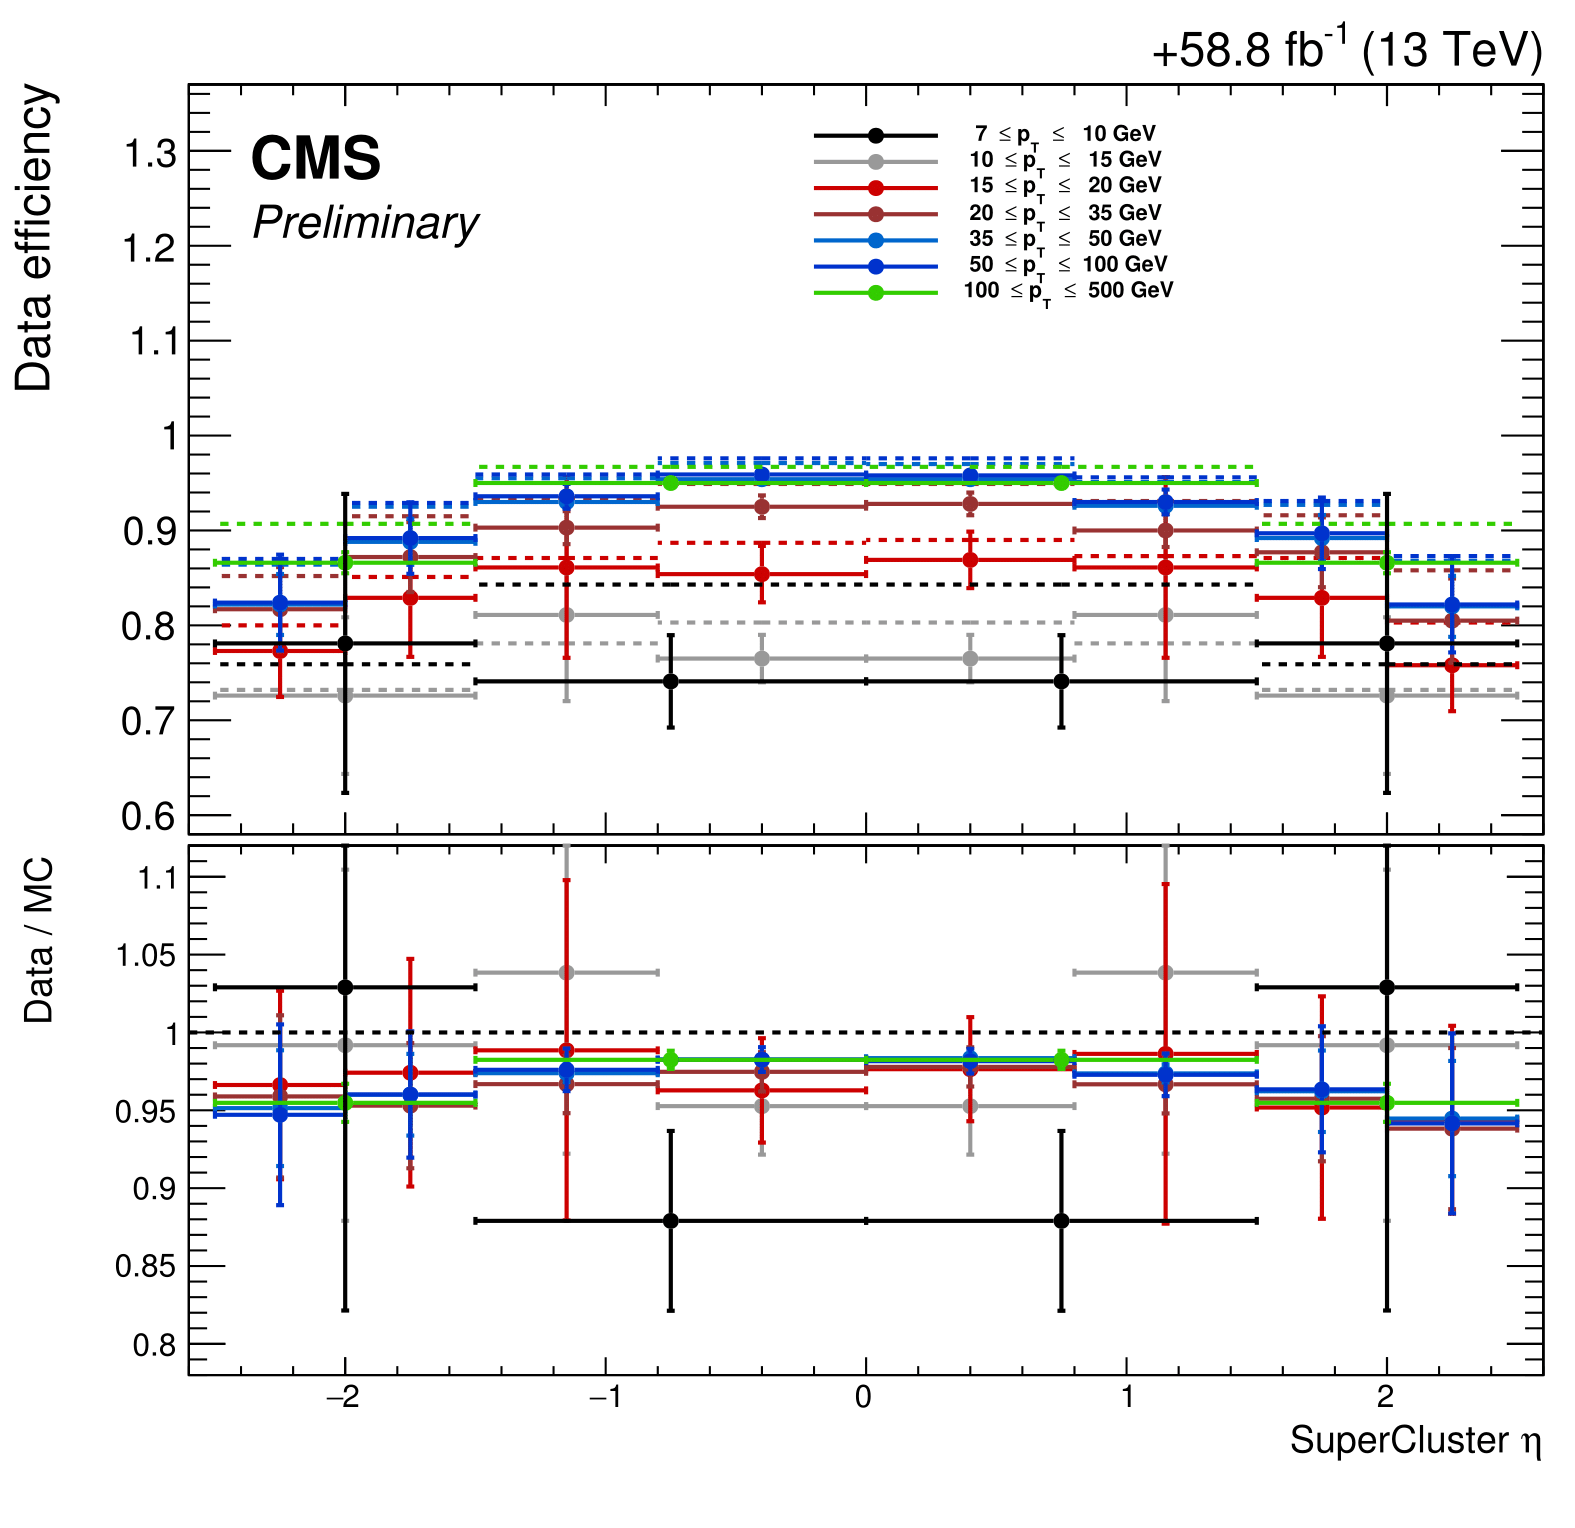
\includegraphics{Figures/Electrons/eleSFvsEta.png}}}
%    \subfigure [] {\resizebox{7.5cm}{!}{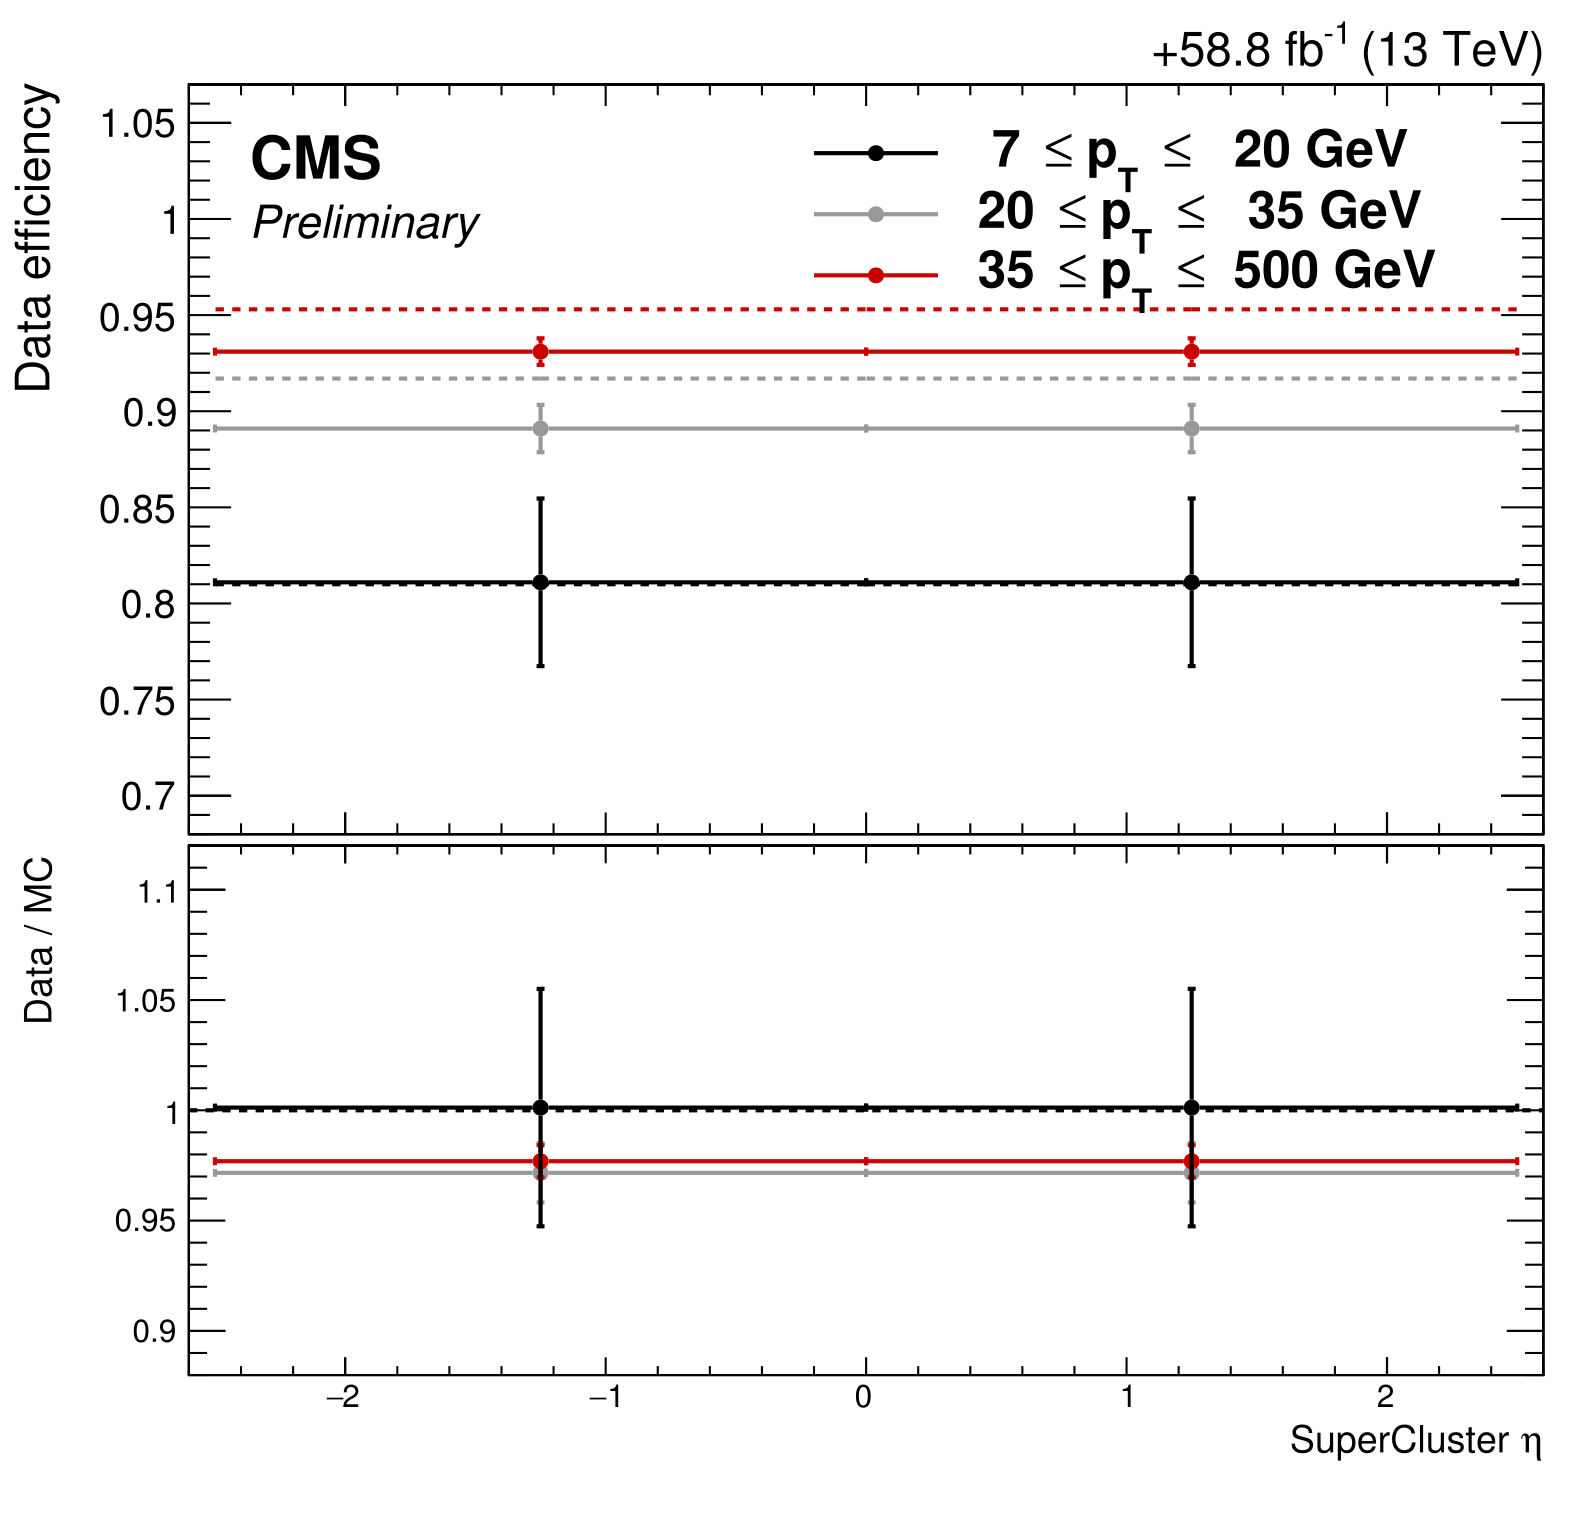
\includegraphics{Figures/Electrons/eleSFvsEtagap.png}}}\\
%\caption{Electron selection efficiencies vs $\eta$, non-gap electrons (left) and gap electrons (right), together wit the corresponding data/MC ratio at the bottom part of each plot.}
%\label{fig:ele_sel_eta_turn_on}
%\end{center}
%\end{figure}
%
%%\begin{figure}[!htb]
%%\begin{center}
%%    \subfigure [] {\resizebox{7.5cm}{!}{
\includegraphics{Figures/Placeholder.png}}}
%%    \subfigure [] {\resizebox{7.5cm}{!}{
\includegraphics{Figures/Placeholder.png}}}\\
%%\caption{2D ($p_T, \eta$) Electron selection Scale Factors measured using the Tag-and-Probe technique described in the text, non-gap electrons (left) and gap electrons (right).}
%%\label{fig:ele_sel_scale_factors}
%%\end{center}
%%\end{figure}
%
%
%%\paragraph{Systematic uncertainties}\mbox{}\\
%%\label{par:Systematic_uncertainties}
%%%%%%%%%%%%%%%%%%%%%%%%%%%%%
%
% The EGM recommendations about evaluation of Tag-and-Probe uncertainties on efficiency measurements are followed. Specifically, we consider
%
%\begin{itemize}
%   \item Variation of the signal shape from a MC shape to an analytic shape (Crystal Ball) fitted to the MC
%   \item Use of analytic function (Crystal Ball) to fit the signal as alternative of MC template %Variation of the background shape from a CMS-shape to a simple exponential in fits to data
%%   \item Variation of the tag selection: tag $p_{T}>$35~GeV and passes MVA-based 8X ID
%   \item Using an NLO MC sample for signal templates
%\end{itemize}
%
%Assessment of total uncertainty for measurement of the scale factors is taken as quadratic sum of statistical uncertainties (returned from the fit) and the aforementioned systematic uncertainties.
%
%
%
